\section{Past Experiments}
\paragraph{}
During the development of the Framework, many small tests have been developed, to both test the capabilities of the framework, and to be used in real studies.
In the following subsections some of those scenes are described.

\subsection[Influence of continuous depth]{Pilot Study: Influence of continuous depth on fatigue\label{FatiguePilot}}
\paragraph{}
Objective of the study is to quantify the effect of a continuous depth element on the time it takes participants to focus objects at various depths, and the change in refocus time with the progression of the experiment.

This study was conducted in parallel with the development of \ER\ and has given immediate feedback for required features and discovered problems.


\begin{center}
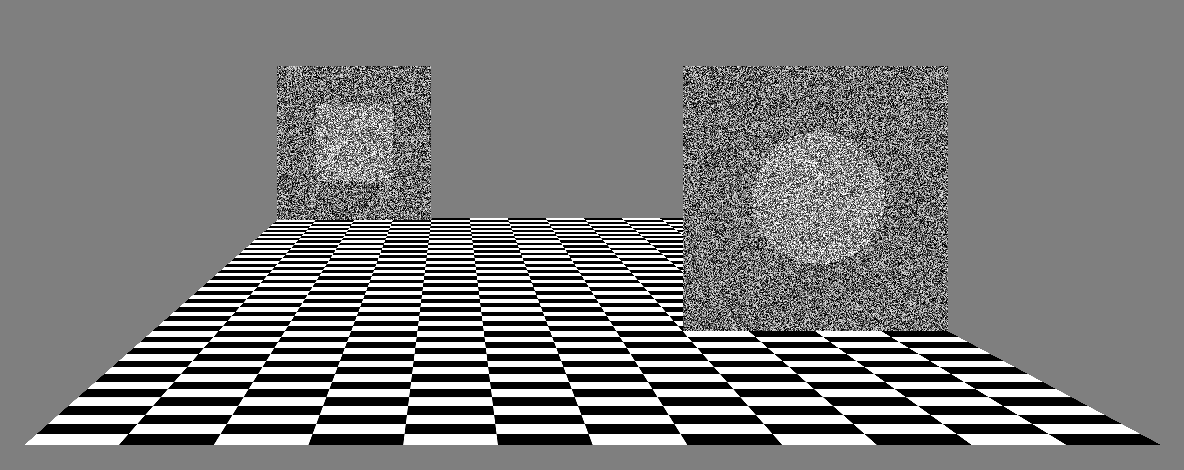
\includegraphics[width=7.5cm]{media/pilotFatigue.png}
\end{center}

\paragraph{Visual}
The test stimulus consists of a grey background (50\% grey), a continuous depth element (plane, checkerboard pattern, averaging in 50\% grey) and two random dot targets (approximately 50\% grey).
The targets show a shape which is either convex (coming out of the screen), or concave (going into the screen).
For the encoding details see section \ref{RDS}. The random pattern consists of eight shades of grey, of which the dark seven are used for the background, and the light seven for the foreground.

The random dot targets are resting on the plane, and border to either the left or the right border.
Each target can be at  one of three depth locations, at a separation of \unit[6]{cm}, \unit[0]{cm} and \unit[-6]{cm} (\unit[-3.1]{°}, \unit[0]{°}, \unit[3.1]{°}).
The targets itself are scaled up in the far position, and scaled down in the near position, to make their apparent size constant.

The image is back-projected on a screen by two projectors through circular polarisation filters.
The image height is \unit[0.79]{m}, it's width is \unit[1.3]{m} (\unit[36]{°} by \unit[22]{°} field of View).
The participant's head is at \unit[2]{m} distance of the screen, and observes the screen with polarised filter goggles. The room is dark.

\paragraph{Mechanics}
To asses the the effect of the continuous depth element, response time is logged.
The other variables are the depth location of the object, the change in depth measured in angular separation, the block number and the presence of the continuous depth element.

The expected input is randomized, so concave and convex targets should be similarly common.
The three depths and the two sides lead to 18 depth changes.

A cycle is built so that every depth change appears exactly once.
This is achieved by pre-computing three cycles and their inverses that visit each of the six positions three times, once from each of the three nodes on the other side.
Such a cycle has 18 steps, and 19 targets.
Cycles are picked at random out of the pre-computed cycles, randomly permuting the depth positions of right and left.
This gives 36 different permutations per cycle, and 216 different permutations overall.

Ten cycles form a block, either with or without continuous depth plane.
The start state is chosen by the tester to counterbalance it, the presence of the depth element in later blocks is alternated.
The whole test contains 12 blocks, 2280 targets.

Before the start, after the end, and after the first six blocks, a questionnaire is presented.
It starts with seven questions, with replies on a scale with six steps.
An other 16 questions require answers on a four step scale.


\subsection{Bisect test\label{Bisect}}
\paragraph{}
This is a helper test for the study on the influence of continuous depth on fatigue.
It's purpose is to find out the limits for stereo vision a person can reach.
During the first pilot study it became obvious that this depends heavily on the individual's experience in stereo viewing.

The test is visually very simple, it only shows one pixel plane with a stereogram.
The complexity is in the code.
(The name comes from the originally proposed algorithm.)

\paragraph{Mechanics}
Unlike usual tests it is not divided in blocks, and it is not limited by number of trials.
The tests are not balanced and pre-randomized either.

Instead the target moves it's position on screen and in depth dependent on the previous answers and the current position.
The target is moved to a near and far point in alternating order.
Five correct replies in a row allow the target point to move further away from the zero parallax plane,
a wrong answer makes it move closer.

The test is stopped when a predetermined maximal limit is reached or a limit is repeatedly failed to be reached.
During the test, voice output announces the current limit.

\subsection{Testing Scene}
\paragraph{}
The testing scene was created to test various stimuli positions and compositions for the study in described in section \ref{FatiguePilot}.
It was used in the design phase, and not for the study itself.
The scene contained a number of targets that could be moved independently in space.
The floor plane visibility was also controllable.
This allowed immediate verification of the test stimulus in fullscreen under experimental conditions.


\section{Future Experiments}
\paragraph{}
Which future experiments will happen is still unsure.
The fatigue experiment described in the previous section will be repeated in a bigger scale, with a bigger screen and increased distance.
This is expected to more closely mimic a cinematic setting with a huge screen.

\paragraph{Pinning}
A test on pinning could improve knowledge of this effect, and possibly provide clues on how such border conflicts can be prevented or mitigated.
Pinning test experiments consisted of rotating objects that were moved to the border of the scene while being in front or behind the parallax plane.
How this could be incorporated in a study is not clear at this time.

\paragraph{Motion Sickness}
A motion sickness test could evaluate how stereoscopic visual information influences the perception of motion, and how it can be tolerated.
It would involve a camera moving on a predefined or random path.
\ER's camera is fully controllable, moving it along a path is easy.
A possible method to define the path would be as b-spline or mathematical function.
A more complex representation could consist of a list of forces applied over time with the path being calculated by calculating physics.

It is worth to note that while \ER\ supports all those methods, there is no direct support for either.
The power of a programming language gives all freedom and all responsibility to the test designer.


\section{Conclusions}
\paragraph{}
I learned a lot during my work on this thesis.
The new technologies I worked with and the new environment has changed my view about programming.
But the most influence on me had the mistakes I made.

From what I know now, I would work differently, start with a more extensive design and try to see early on how the finished product will look like.
This was not possible since at the start of the thesis, the requirements were not clearly defined.
Only through experimenting and speaking with potential users the requirements could be specified in detail.

My first goal was to get a working prototype to perform experiments with.
The study on the effect of continuous depth on fatigue was successfully conducted with the prototype, which was later extended.
The result of this continuous extension process is a design that, while flexible and extensible, suffers some artefacts of the past.
The tight integration of lua and the scene graph and the union of creator and execution environment might complicate future extension.

\paragraph{}
Overall I am happy with the result.
\ER\ does what was expected and more.
It has proven itself in practical use, the results of the first study have deepened our understanding of stereoscopic viewing fatigue.

The questions asked at the beginning of the thesis were answered.
Many of the methods to simplify scene creation are integrated in \ER and
simple test visuals can easily generated by placing objects in a scene.

User-friendliness in the traditional areas of the test design is however lacking.
Where traditional applications expect the test visuals to be generated externally and focus on putting them together in a simple user interface, \ER\ relies on a scripting language to define the test.
Simplicity is partially gained by sacrificing power, a compromise not yet taken in \ER.
It might be worthwhile to give away the freedom of a scripting language for the ease-of-use of a traditional test generator.

\clearpage

\subsection*{Thanks}
\paragraph{}
I thank Steven Poulakos who helped me with feedback and beta testing of prototypes during his fatigue study and proof reading the thesis.

Cary Kornfeld for allowing me to work on this project and continuous emphasis on creating code that is maintainable and well commented.

